\documentclass{examnotes}

\newcommand{\E}{\Epsilon}
\newcommand{\Var}{\mathrm{Var}}
\newcommand{\Cov}{\mathrm{Cov}}

\usepackage{sectsty}
\sectionfont{\Large\raggedright}
\subsectionfont{\raggedright}

\header{STA2603 Distribution Theory II}
%%%%%%%%%%%%%%%%%%%%%%%%%%%%%%%%%%%%%%%
\begin{document}

\obeylines

\h{STA2603 Distribution Theory II}

{\red{Always specify the domain of the function!}} \hfill  {\red{Always specify the parameters when identifying the distribution!}}

%%%%%%%%%%%%%%%%%%%%%%%%%%%%%%%%%%%%%%%
\h{Study Unit 2}

Frequency Function (discreet) = density function (continuous).
Distribution functions is CDF.

\h{Discreet Random Variables}

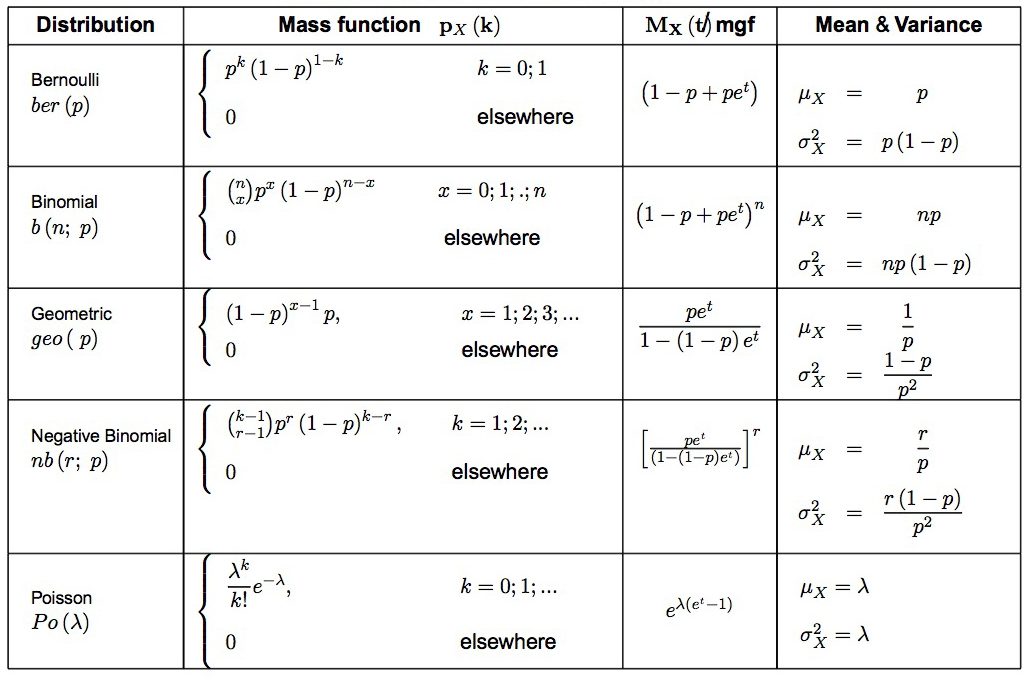
\includegraphics[scale=0.5]{./img/disscreet.jpg}

\disobeylines
Hypergeometric :
\mymath{p(x)=\begin{cases} \displaystyle\frac{\binom{r}{x}\binom{n-r}{m-x}}{\binom{n}{m}} & \text{if }x=0,1,2,\dots.n\\
0 & \text{otherwise}
\end{cases}
} %\mymath
\obeylines

Probability of x successes in a sample size $m$ from sample space $n$ and a subset $r$  

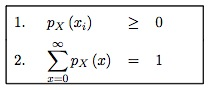
\includegraphics[scale=0.8]{./img/2dis.jpg}

$\binom{n}{x} = \displaystyle\frac{n!}{x!(n-x)!}$

\sh{Bernoulli Random Variables}

\vspace{6pt}

\disobeylines
Indicator random variable \mymath{I_A(\omega)=\begin{cases} 1 & \omega \in A\\
0 & \text{otherwise}
\end{cases}
} %\mymath
\obeylines

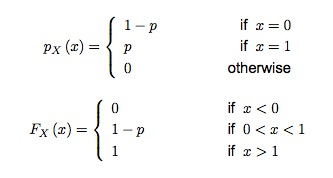
\includegraphics[scale=0.6]{./img/2ber.jpg}

\sh{Binomial Distribution}

The sum of independent Bernoulli variables is a binomial random variable. 
To prove binomial probabilities sums to 1. Use finite binomial series expansion:
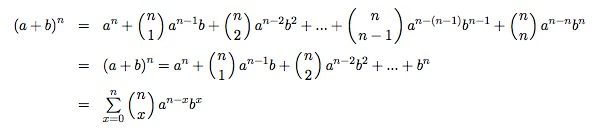
\includegraphics[scale=0.7]{./img/2ber2.jpg}
\vspace{-10pt}
and therefore it is a series expansion of $[(1-p)+p]^n$
\vspace{6pt}
\sh{Geometric Distribution}

To prove that geometric distribution sums to 1, use Taylor series at x=0
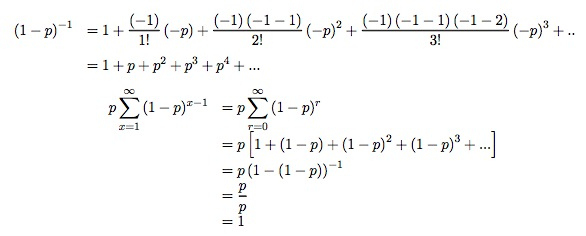
\includegraphics[scale=0.7]{./img/2geo.jpg}

\sh{Negative Binomial Distribution}

A negative binomial random variable can be expressed as the sum of \emph{r} independent geometric variables.

{\sh{Hypergeometric distribution}
\vspace{6pt}

\disobeylines
\mymath{pX(x)=\begin{cases} \displaystyle\frac{\binom{r}{x}\binom{n-r}{m-x}}{\binom{n}{m}} & \text{if }x=0,1,2,\dots.n\\
0 & \text{otherwise}
\end{cases}
} %\mymath

\obeylines

\sh{Poisson Distribution}

To show it is a frequency function: 

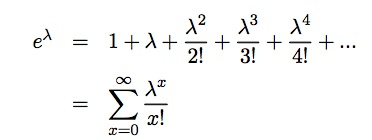
\includegraphics[scale=0.7]{./img/2poi1.jpg}
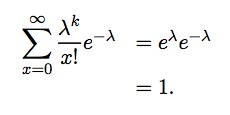
\includegraphics[scale=0.7]{./img/2poi2.jpg}

Poisson distribution can be used to approximate binomial distribution, if \emph{n} is large and \emph{p} is small.

\h{Continuous Random Variables}

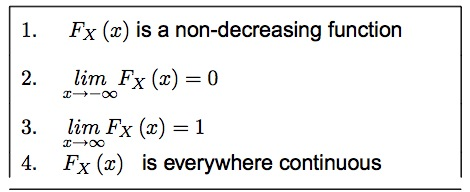
\includegraphics[scale=0.7]{./img/2con1.jpg}
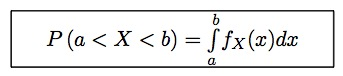
\includegraphics[scale=0.7]{./img/2con2.jpg}
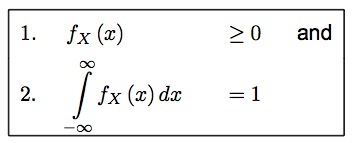
\includegraphics[scale=0.7]{./img/2con3.jpg}
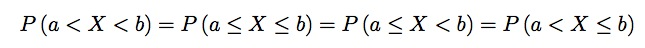
\includegraphics[scale=0.7]{./img/2con4.jpg}

The $p$th quantile: $F(x_p)=p$ \quad or $P(X\le x_p)=p$ \quad and $x_p=F^{-1}(p)$

\sh{Exponential Density}

\sh{Gamma Density}

Gamma function $\Gamma(a)=\displaystyle\int_0^\infty{x^{a-1}e^{-x}}$ \quad Properties $\Gamma(\alpha+1)=\alpha\Gamma(\alpha)$ \quad $\Gamma(\frac{1}{2})=\sqrt{\pi}$
\quad $c^n\Gamma(n)=\displaystyle\int_0^\infty{x^{n-1}e^{-\displaystyle\frac{x}{c}}}$

$\Gamma(2) = 1$ \vspace{6pt}

If $\alpha=1$ then it becomes exponential density
If $\lambda=1$ then it is a one parameter gamma density

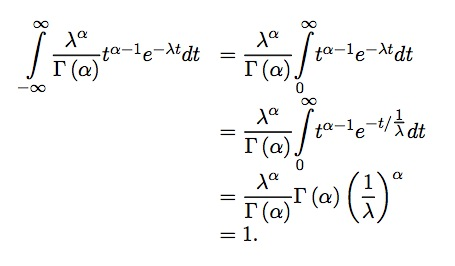
\includegraphics[scale=0.4]{./img/2gam.jpg}

\sh{Normal (Gaussian) distribution}

\sh{Beta Density}

Beta function: $B(m,n)=\displaystyle\int_0^1{x^{m-1}(1-x)^{n-1}dx}$ \quad or $B(m,n)=\displaystyle\int_0^\infty{\frac{x^{n-1}}{(1+x)^{m+n}}dx}$

To prove density function:

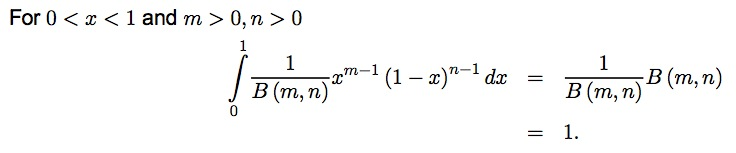
\includegraphics[scale=0.4]{./img/2bet2.jpg}
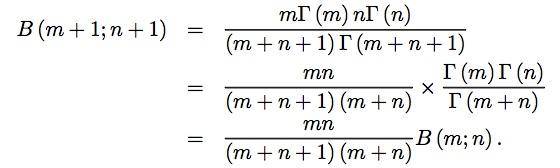
\includegraphics[scale=0.4]{./img/2bet3.jpg}
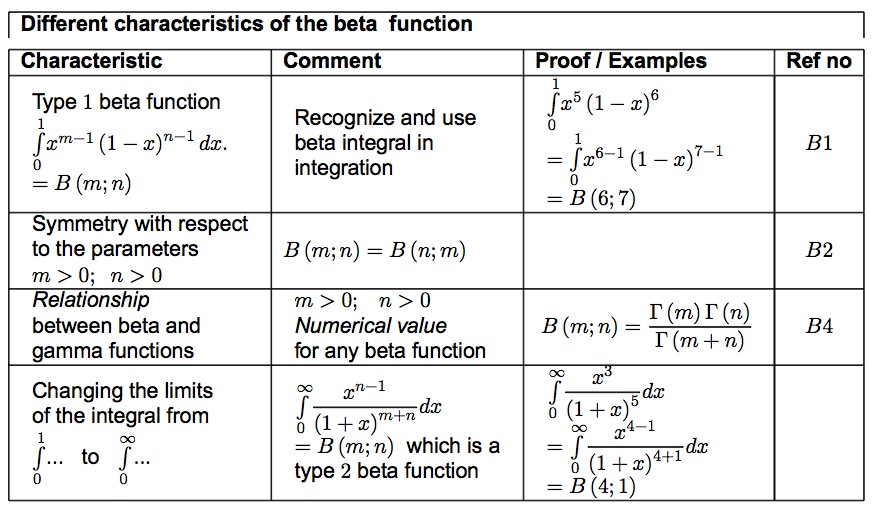
\includegraphics[scale=0.5]{./img/2bet1.jpg}

\sh{Cauchy Density}

\disobeylines

\mymath{f(x)=\frac{1}{\pi}\left( \frac{1}{1+x^2}\right) \quad -\infty < x < \infty
} %\mymath
\obeylines

\h{Functions of random Variables}

Standard normal CDF $= \Phi(X)$ \quad Standard normal density $= \varphi(X)$

{\bf Proposition A:}
if $X\mytilde N(\mu,\sigma^2)$ and $Y=aX+b$, then $Y\mytilde N(a\mu+b,a^2\sigma^2)$

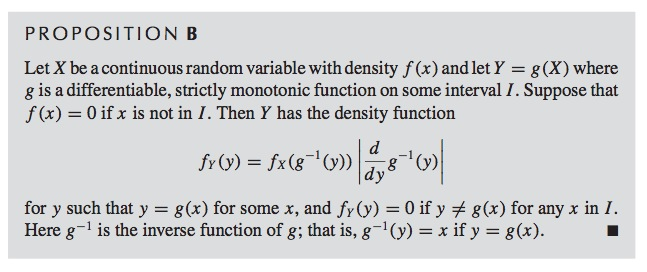
\includegraphics[scale=0.6]{./img/2fun1.jpg}
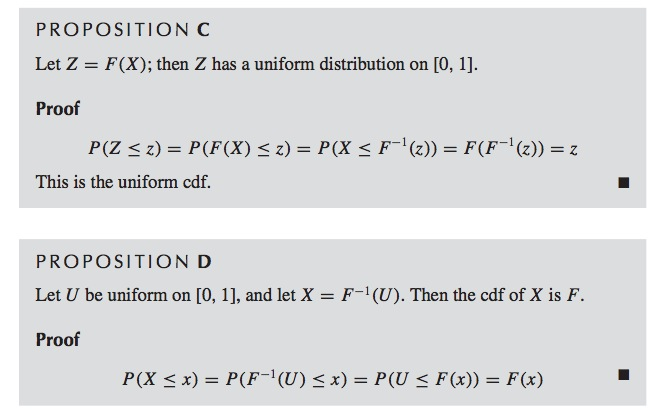
\includegraphics[scale=0.6]{./img/2fun2.jpg}

$[N(0,1)]^2\mytilde \chi^2_1$

Weibull density: $\displaystyle\frac{\beta}{\alpha^\beta}x^{\beta-1}e^{-\left(\displaystyle\frac{x}{\alpha}\right)^\beta}$

%%%%%%%%%%%%%%%%%%%%%%%%%%%%%%%%%%%%%%%
\h{Study Unit 3}

\sh{Discreet Random Variables}

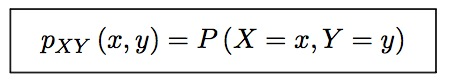
\includegraphics[scale=0.4]{./img/3jd1.jpg}
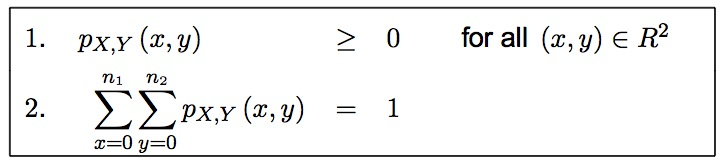
\includegraphics[scale=0.4]{./img/3jd2.jpg}

\sh{Continuous Random Variables}

Marginal density.

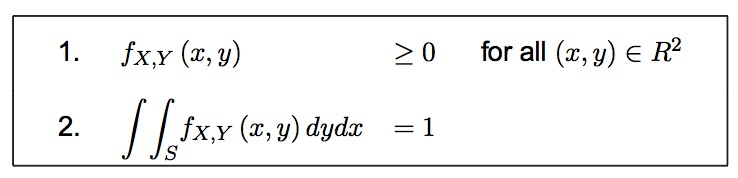
\includegraphics[scale=0.4]{./img/3con1.jpg}                                         
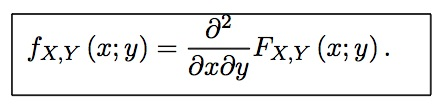
\includegraphics[scale=0.4]{./img/3con2.jpg}                                         
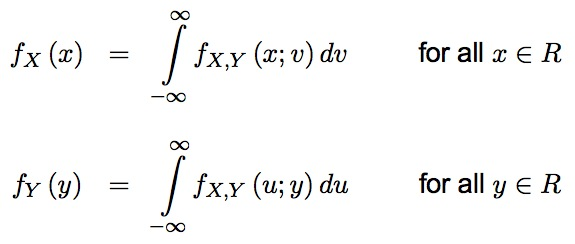
\includegraphics[scale=0.4]{./img/3con3.jpg}                                         

\red{Marginals sum to 1}

Joint cumulative distribution.

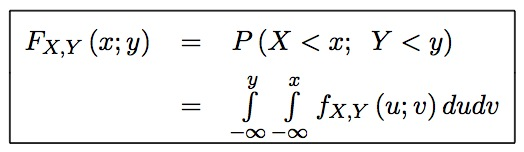
\includegraphics[scale=0.4]{./img/3con4.jpg}                                         

\sh{Independent Random variables}

Independent if $F(x,y)=F_X(x)F_Y(y)$

Two discreet random variables will be independent if th their joint mass function factors.

\sh{Conditional Distributions}

Discreet:

The law of total probability. $p_X(x)=\displaystyle\sum_y{p_{X|Y}(x|y)p_Y(y)}$

Continuous:

The law of total probability. $f_Y(y)=\displaystyle\int_{-\infty}^\infty{f_{Y|X}(y|x)f_X(x)\,dx}$

%%%%%%%%%%%%%%%%%%%%%%%%%%%%%%%%%%%%%%%
\h{Study Unit 4}
\sh{Expected Value of Random Variables}

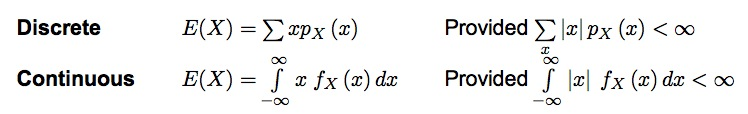
\includegraphics[scale=0.5]{./img/41.jpg}

\sh{Markov's Inequality}
$P(X\ge t)\le \frac{\Epsilon(X)}{t}$

\sh{Expectations of functions of random variables}
\ra Corollary A:  $\E(XY)=\E(X)\E(Y)$

\sh{Expectations of linear combinations of random variables}
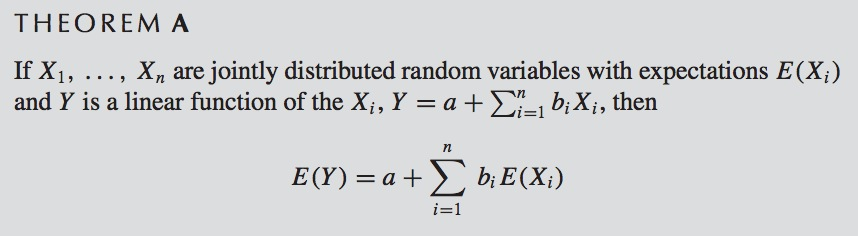
\includegraphics[scale=0.4]{./img/412A.jpg}

\ra Proof for $n=2$: 
\rn{1} Write out full expectation
\rn{2} Multiply out and separate integrals
\rn{3} First sums to 1
\rn{4} Second/third sum to expected values
\rn{5} State integral is convergent

\sh{Variance and standard deviation}

$Var(X)=\E\left([X-\E(X)]^2\right) $
$Var(X)=\E(X^2)-\left[E(X)\right]^2$

\vspace{6pt}
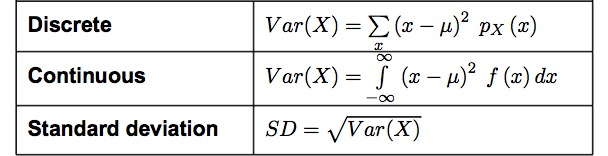
\includegraphics[scale=0.4]{./img/42.jpg}

\vspace{6pt}
{\bf Chebyshev's Inequality}: There is a high probability that $X$ will deviate little from its mean if the variance is small.
\vspace{6pt}
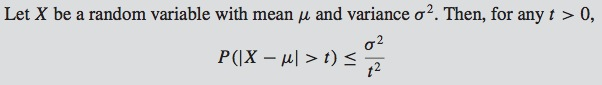
\includegraphics[scale=0.5]{./img/421.jpg}
Setting $t=k\sigma$ then $P(|X-\mu|\ge k\sigma)\le \displaystyle\frac{1}{k^2}$ or what ever is asked.

\sh{Covariance}
\disobeylines
\mymath{Cov(X,Y) &= \E(X-\mu_X)(Y-\mu_Y) \\
&= \E(X,Y)-\E(X)\E(Y)
} %\mymath
\obeylines
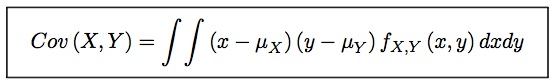
\includegraphics[scale=0.5]{./img/43.jpg}

If independent then: $ \E(XY)=\E(X)\E(Y)$ and covariance is $0$

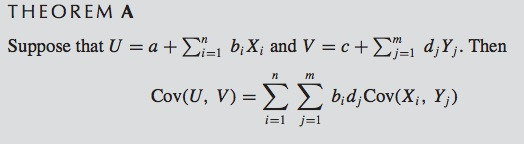
\includegraphics[scale=0.5]{./img/431.jpg}
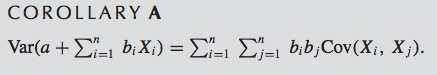
\includegraphics[scale=0.5]{./img/432.jpg}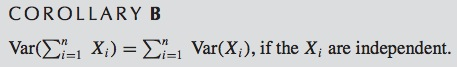
\includegraphics[scale=0.5]{./img/433.jpg}

\disobeylines
\mymath{\Var(X+Y)&=\Cov(X+Y,X+Y) \\
&       =\Var(X) + \Var(Y) + 2\Cov(X,Y)
} %\mymath

\obeylines
$\E\left(\displaystyle\sum X_i\right)=\sum \E(X_i)$
\vspace{6pt}
$\Var\left(\displaystyle\sum X_i\right)=\sum \Var(X_i)$ if $X_i$ are independent.

\sh{Correlation coefficient}
\note{\Large Revise Properly!!!!!!}

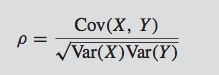
\includegraphics[scale=0.5]{./img/434.jpg}

\sh{Conditional Expectation and Prediction}
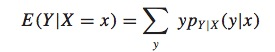
\includegraphics[scale=0.5]{./img/441.jpg}
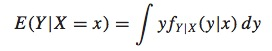
\includegraphics[scale=0.5]{./img/442.jpg}
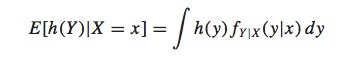
\includegraphics[scale=0.5]{./img/443.jpg}


{\bf Law of total expectation}
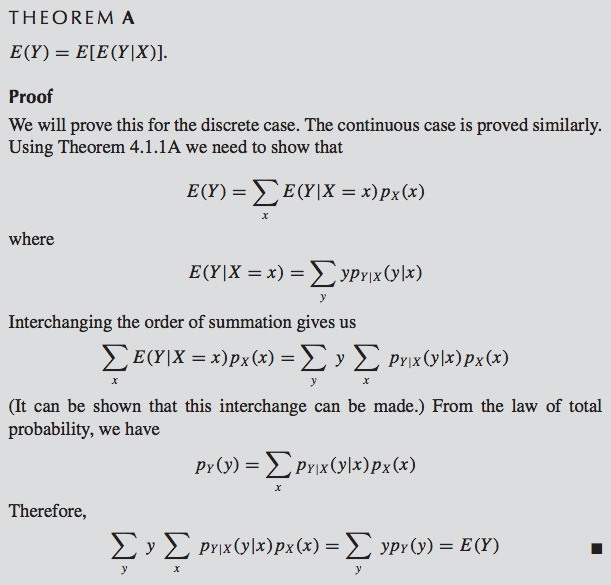
\includegraphics[scale=0.5]{./img/44A.jpg}


\sh{Moment-generating functions}
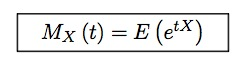
\includegraphics[scale=0.5]{./img/451.jpg}
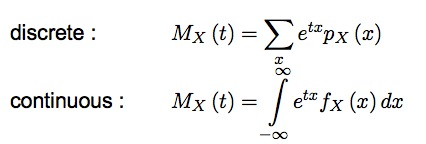
\includegraphics[scale=0.5]{./img/452.jpg}
\ra Same mgf then same distribution.
\ra If the mgf can be determined it can be uniquely determines then probability distribution. 
\ra The mgf provides an elegant way to compute the moments of a distribution.

\vspace{6pt}
\ssh{Calculating moments}
\ra First principles
\vspace{6pt}
\rna Discreet: $\E(X^r)=\displaystyle\sum x^rp_X(x)$
\vspace{6pt}
\rna Continuous:  $\E(X^r)=\displaystyle\int x^rf_X(x)$
\vspace{6pt}
\ra Using moment-generating function
\vspace{6pt}
\rna $M^{(r)}(0)=E(X^r)$ 
\ra Using Taylor series expansion 
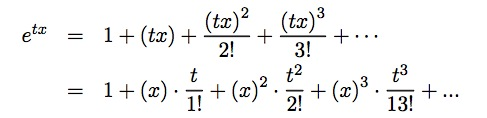
\includegraphics[scale=0.5]{./img/454.jpg}


%%%%%%%%%%%%%%%%%%%%%%%%%%%%%%%%%%%%%%%
\h{Study Unit 5}



%%%%%%%%%%%%%%%%%%%%%%%%%%%%%%%%%%%%%%%
\h{Study Unit 6}















\end{document}
